\documentclass[a4paper]{article}

\usepackage[czech]{babel} %https://github.com/michal-h21/biblatex-iso690
\usepackage[
   backend=biber      % if we want unicode 
  ,style=iso-numeric % or iso-numeric for numeric citation method          
  ,babel=other        % to support multiple languages in bibliography
  ,sortlocale=cs_CZ   % locale of main language, it is for sorting
  ,bibencoding=UTF8   % this is necessary only if bibliography file is in different encoding than main document
]{biblatex}

\usepackage[utf8]{inputenc}
\usepackage{fancyhdr}
\usepackage{amsmath}
\usepackage{amssymb}
\usepackage[left=2cm,right=2cm,top=2.5cm,bottom=2.5cm]{geometry}
\usepackage{graphicx}
\usepackage{pdfpages}
\usepackage{url}

\usepackage{siunitx}
\sisetup{locale = DE}  %, separate-uncertainty = true    kdybych chtel +/-

\usepackage{float}
\newfloat{graph}{htbp}{grp}
\floatname{graph}{Graf}
\newfloat{tabulka}{htbp}{tbl}
\floatname{tabulka}{Tabulka}

\renewcommand{\thefootnote}{\roman{footnote}}

\pagestyle{fancy}
\lhead{Praktikum IV - (A24) Určování chemického složení materiálů pomocí energiově disperzní analýzy rentgenových spekter}
\rhead{Vladislav Wohlrath}
\author{Vladislav Wohlrath}

\bibliography{source}

\begin{document}

\begin{titlepage}
\includepdf[pages={1}]{./graficos/424-tit.pdf}
\end{titlepage}

\section*{Pracovní úkoly}
\begin{enumerate}
\item ÚKOLY
\end{enumerate}

%Teoretická část
\section*{Teoretická část}
Skenovací elektronový mikroskop používá ke studiu vzorku zaostřený svazek elektronů.
V detektoru Augerových a sekundárních elektronů (SE) vidíme topografický povrch vzorku. Sekundární elektrony jsou elektrony vyražené ze vzorku a od primárních elektronů (PE) je poznáme tak, že mají mnohem menší energii (do cca \SI{50}{\eV}).
V detektoru zpětně odražených vzorků (BSE) vidíme Z-kontrast (atomové číslo), tedy kontrast mezi oblastmi prvků s velmi odlišným atomovým číslem. Vyšší Z znamená vyšší intenzitu BSE (tedy světlejší barvu na snímku). BSE mají energii srovnatelnou s energií PE.

Po dopadu PE na vzorek vzniká RTG záření dvojího druhu. Za prvé je to bzdné záření se spojitým spektrem, které budeme v našem experimentu filtrovat a nijak ho nevyužijeme, a za druhé je to charakteristické záření přítomných prvků s diskrétním spektrem. Každý prvek má charakteristické spektrum, které odpovídá energetickým přechodům při deexcitaci. Podle tohoto spektra dokážeme prvek ve vzorku identifikovat a určit jeho koncentraci.

Při kvantitativní analýze RTG spektra musíme brát v úvahu různé jevy, které se projeví na intenzitě spektrálních čar (korekce na atomové číslo, absorbce, fluorescence) \cite{skripta}. Naštěstí software dodávaný s mikroskopem tyto korekce provádí za nás.

%Podmínky a měřící přístroje
\section*{Podmínky a použité přístroje}

%Výsledky měření
\section*{Výsledky měření}
PE byly urychlené napětím $U=\SI{20}{\kV}$. de Broglieho vlnová délka je
\begin{equation*}
\lambda_{\text{PE}} = \frac{h}{\sqrt{2MUq}}=\SI{8.7}{\pico\metre} \,.
\end{equation*}

Pozorovali jsme tři vzorky:
\begin{enumerate}[noitemsep]
\item slovenská mince
\item neznámý vzorek
\item česká mince
\end{enumerate}
budeme je důsledně nazývat těmito čísly.

Na snímcích z mikroskopu je vždy levá část z detektoru SE a pravá z BSE.

Snímky vzorku 1 při různém zvětšení jsou na obrázcích \ref{o:vz1_01} a \ref{o:vz1_05}.


\begin{figure}[htbp]
\centering
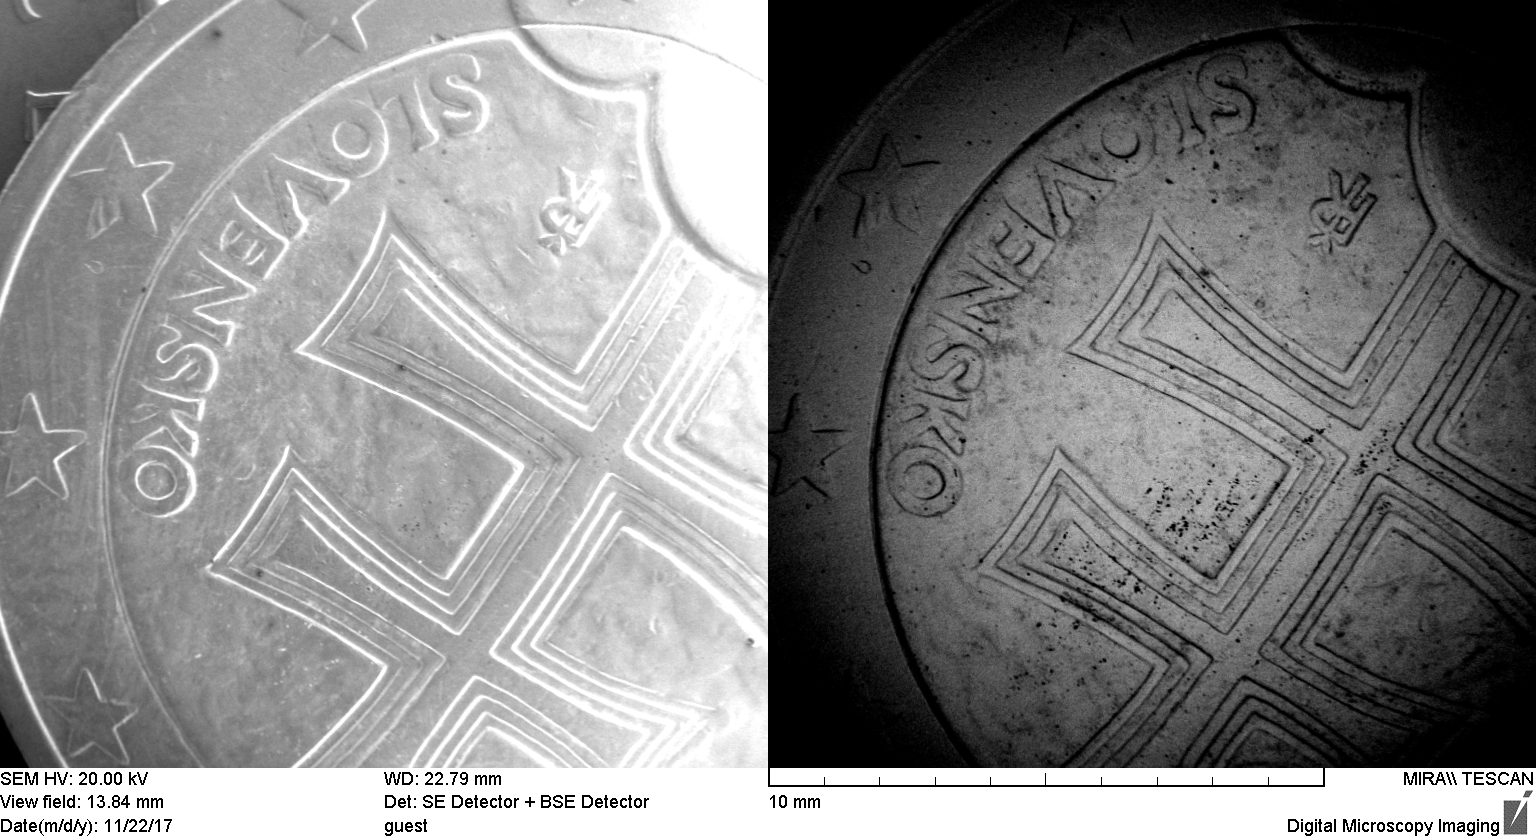
\includegraphics[width=\textwidth-2cm]{graficos/VZ01_01.png}
\caption{Vzorek 1}
\label{o:vz1_01}
\end{figure}
\begin{figure}[htbp]
\centering
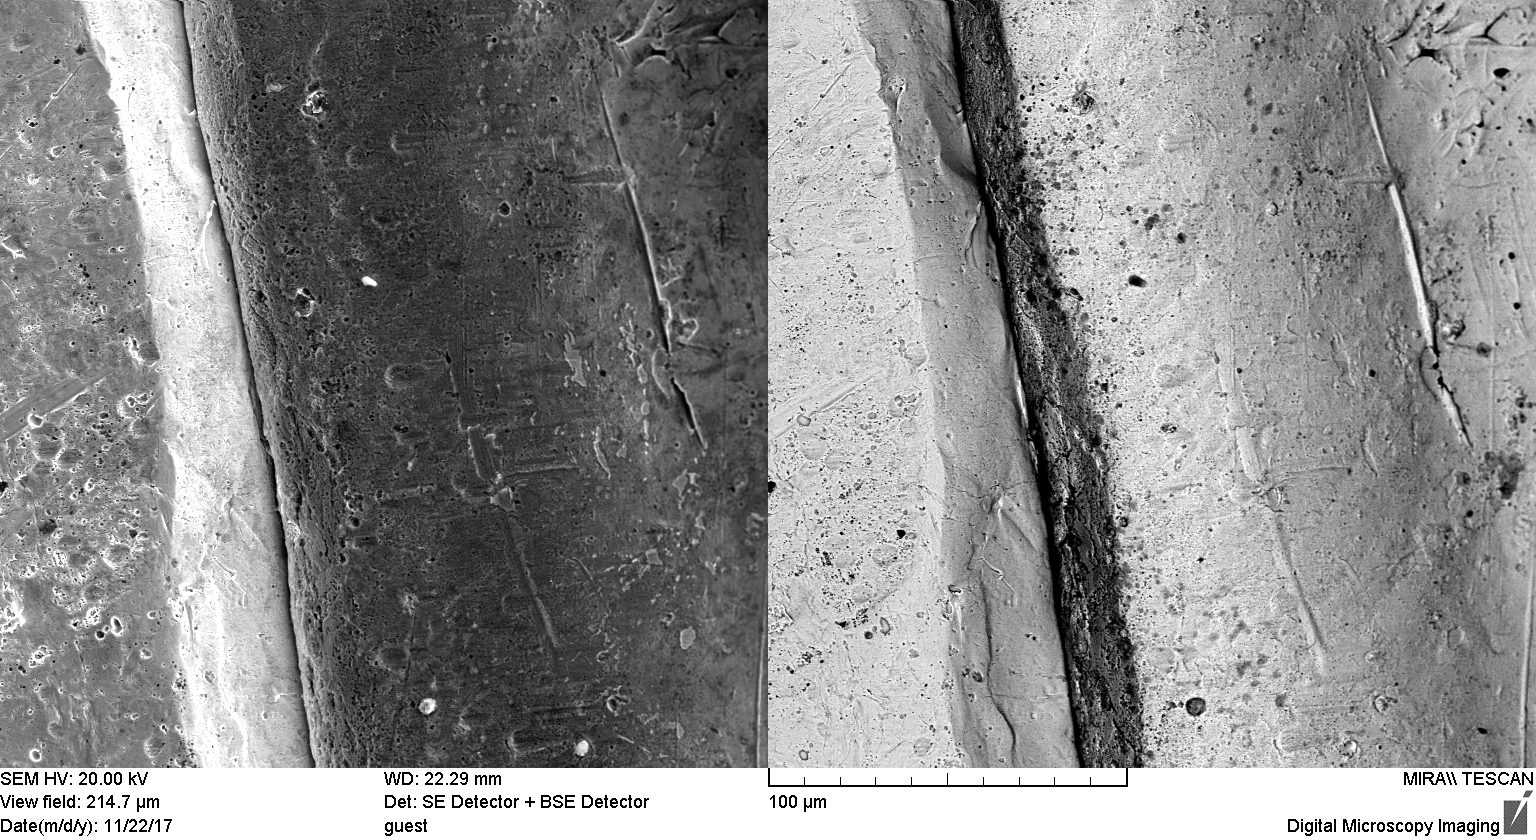
\includegraphics[width=\textwidth-2cm]{graficos/vz01_5.png}
\caption{Vzorek 1}
\label{o:vz1_05}
\end{figure}




U vzorku 2 (viz obrázek \ref{o:vz2_01}) pozorujeme kompoziční kontrast, zřejmě se skládá ze dvou fází. 
Vybrali jsme dvě místa na vzorku, bod A ve světlé oblasti BSE snímku a bod B v tmavé. 
V obou místech jsme provedli kvantitaviní analýzu RTG spektra a určili chemické složení (viz tabulky \ref{t:vz02_a} a \ref{t:vz02_b} a obrázky \ref{o:vz2_a} a \ref{o:vz2_b}). V bodě A je narozdíl od bodu B kromě hliníku přítomna těžší měď, což odpovídá tomu, že těžší prvky mají vyšší intenzitu zpětně odražených elektronů.
Dále jsme provedli lineární sken, který zde neuvádíme, a 2D sken (obrázek \ref{o:vz2_2D}).

\begin{figure}[htbp]
\centering
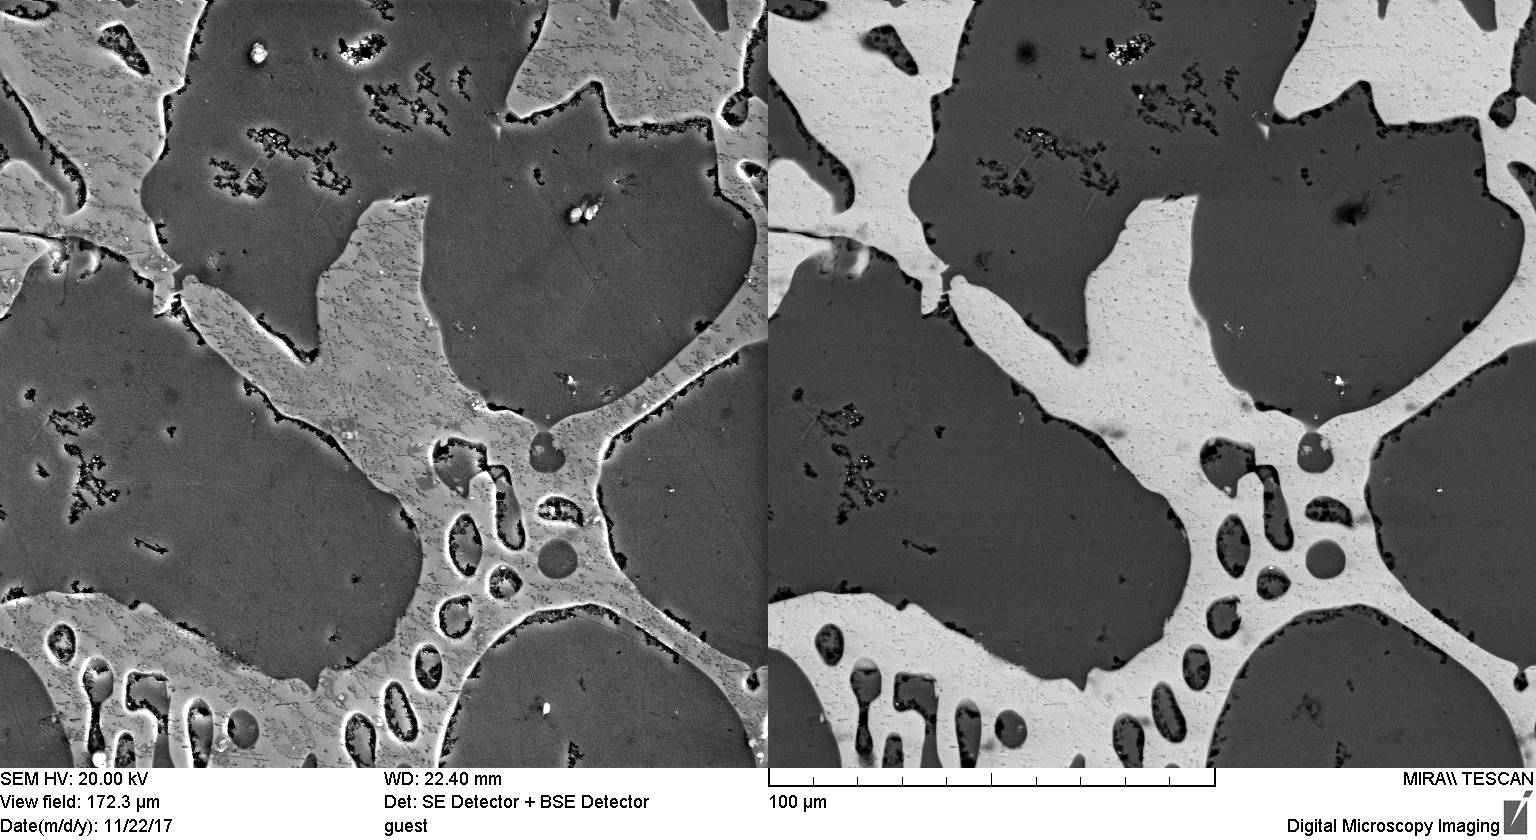
\includegraphics[width=\textwidth-2cm]{graficos/Vz02_01.png}
\caption{Vzorek 2}
\label{o:vz2_01}
\end{figure}

\begin{tabulka}[htbp]
\centering
\begin{BVerbatim}
Spectrum: Ti_Gl_1 13

Element    Series   unn. C norm. C Atom. C Error
                   [wt.-%] [wt.-%] [at.-%]   [%]
------------------------------------------------
Aluminium K-series   46,62   47,37   67,95   2,3
Copper    K-series   51,80   52,63   32,05   1,4
------------------------------------------------
            Total:   98,42  100,00  100,00
\end{BVerbatim}
\caption{Chemické složení vzorku 2 v místě A}
\label{t:vz02_a}
\end{tabulka}

\begin{figure}[htbp]
\centering
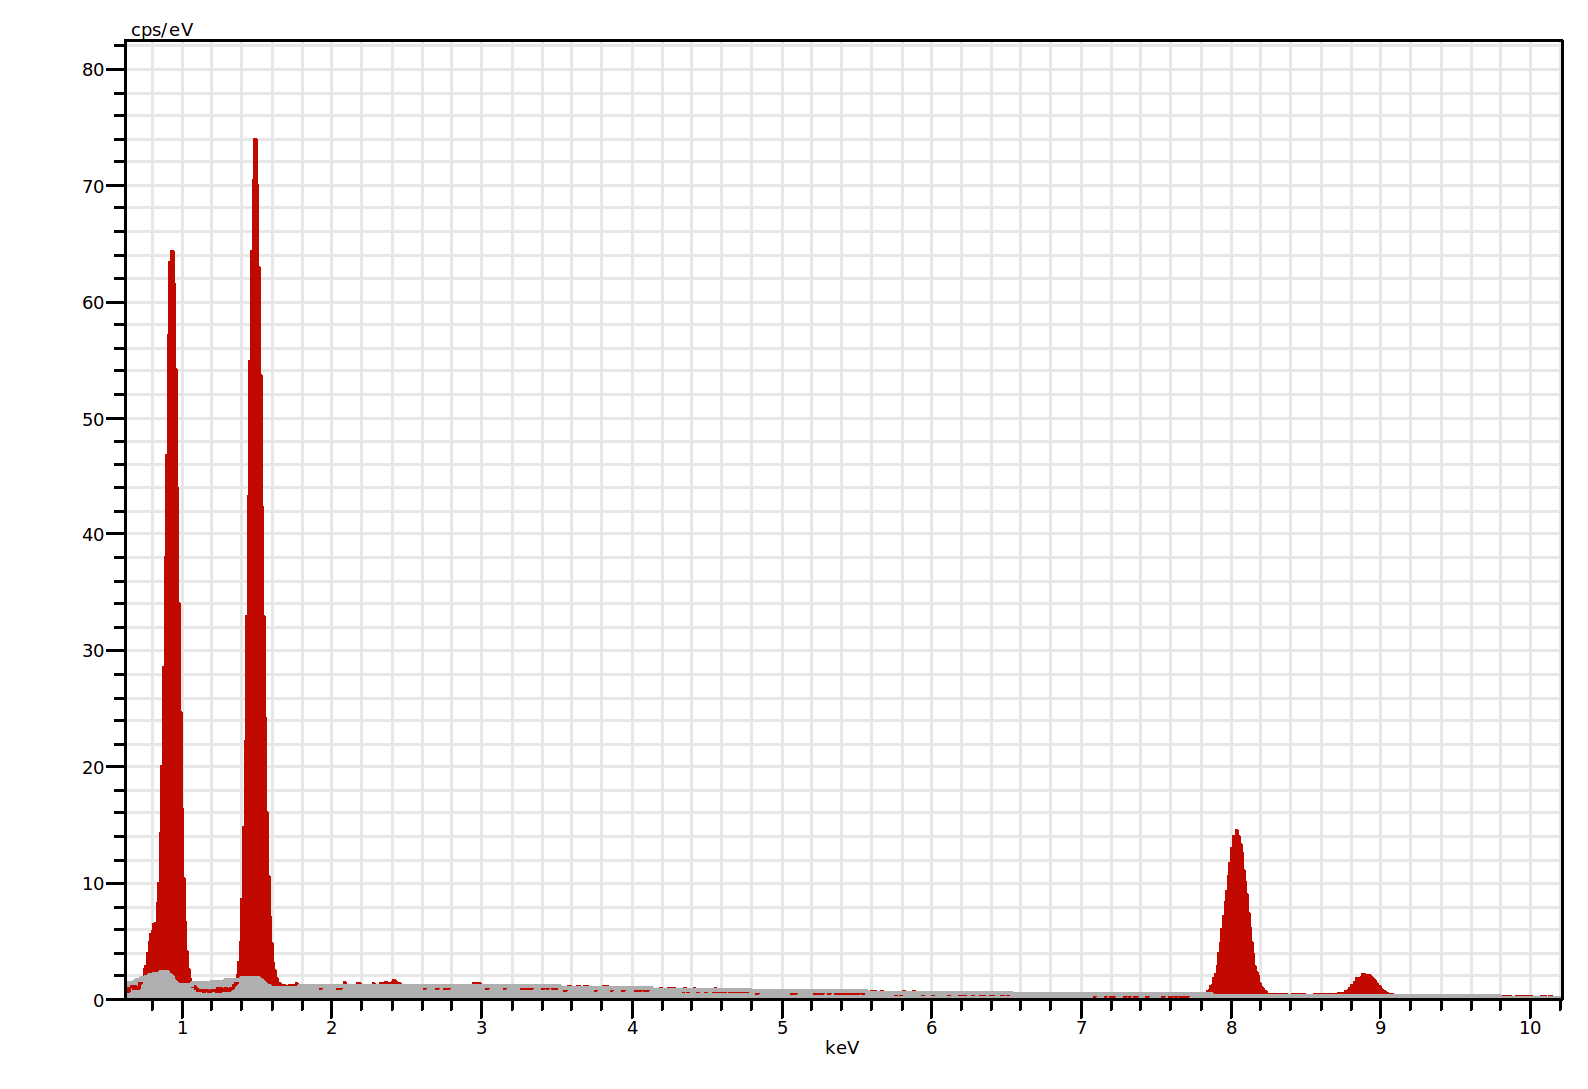
\includegraphics[width=12cm]{graficos/vz2_a.png}
\caption{Spektrum vzorku 2 v místě A}
\label{o:vz2_a}
\end{figure}

\begin{tabulka}[htbp]
\centering
\begin{BVerbatim}
Spectrum: Ti_Gl_1 14

Element    Series   unn. C norm. C Atom. C Error
                   [wt.-%] [wt.-%] [at.-%]   [%]
------------------------------------------------
Copper    K-series    5,30    4,99    2,18   0,2
Aluminium K-series  101,04   95,01   97,82   4,8
------------------------------------------------
            Total:  106,34  100,00  100,00
\end{BVerbatim}
\caption{Chemické složení vzorku 2 v místě B}
\label{t:vz02_b}
\end{tabulka}

\begin{figure}[htbp]
\centering
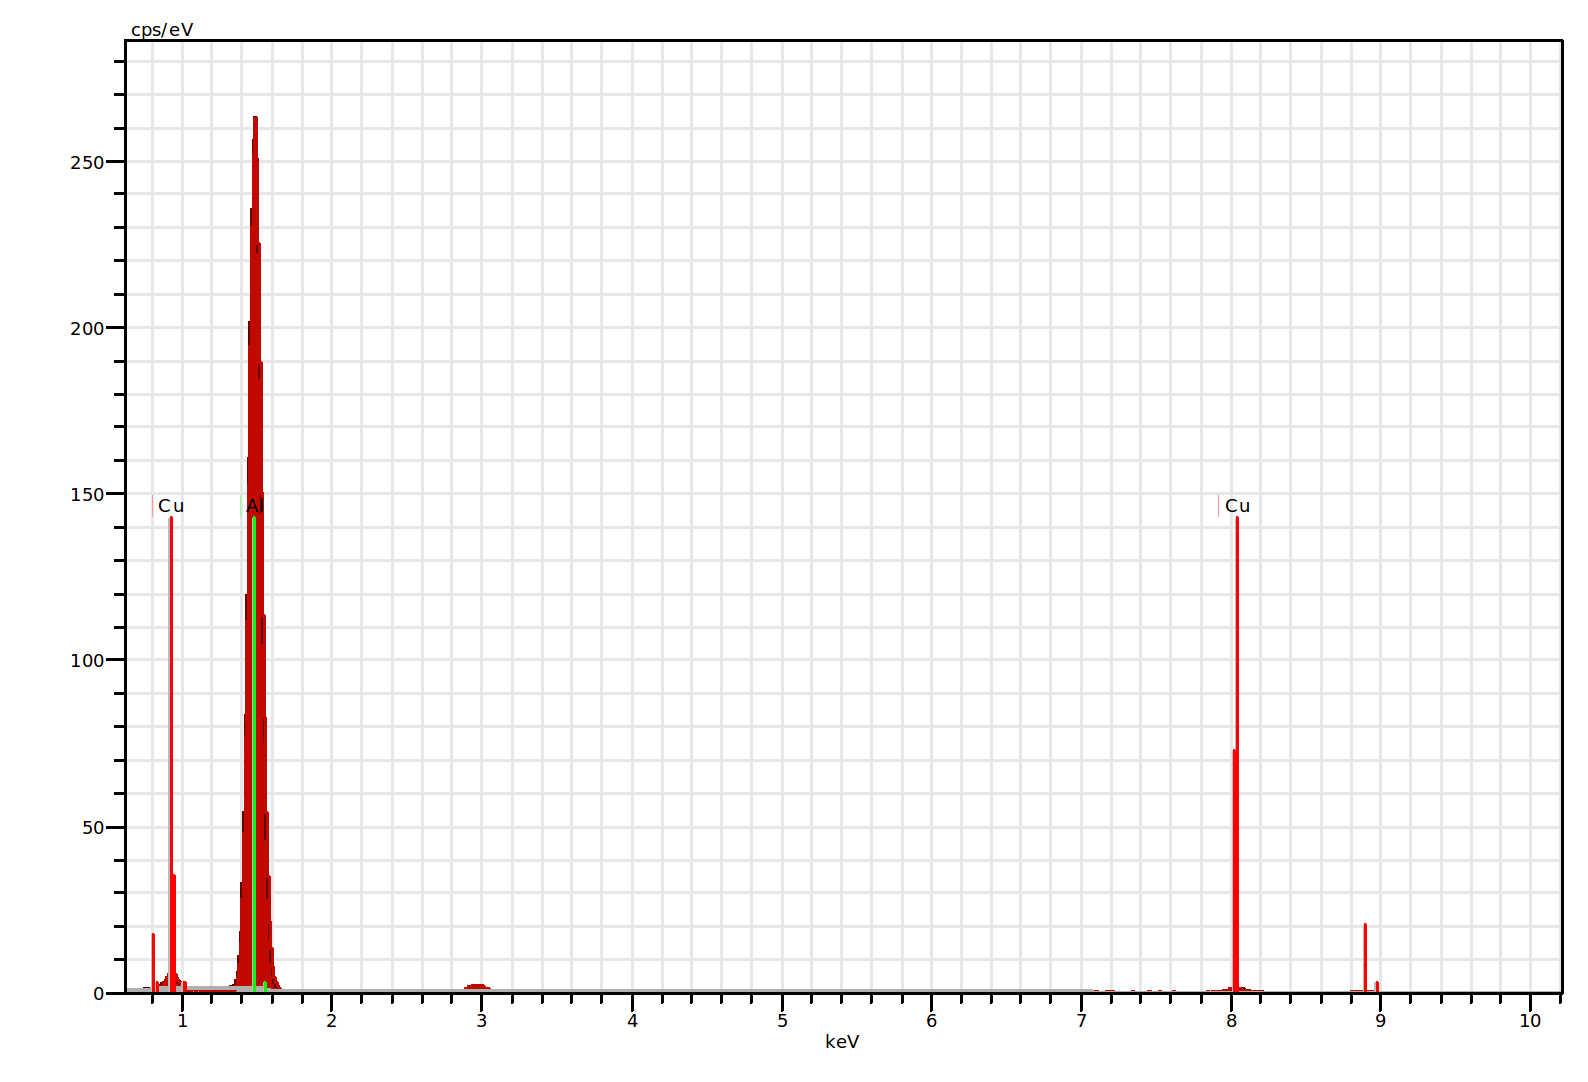
\includegraphics[width=12cm]{graficos/vz2_b.png}
\caption{Spektrum vzorku 2 v místě B}
\label{o:vz2_b}
\end{figure}

\begin{figure}[htbp]
\centering
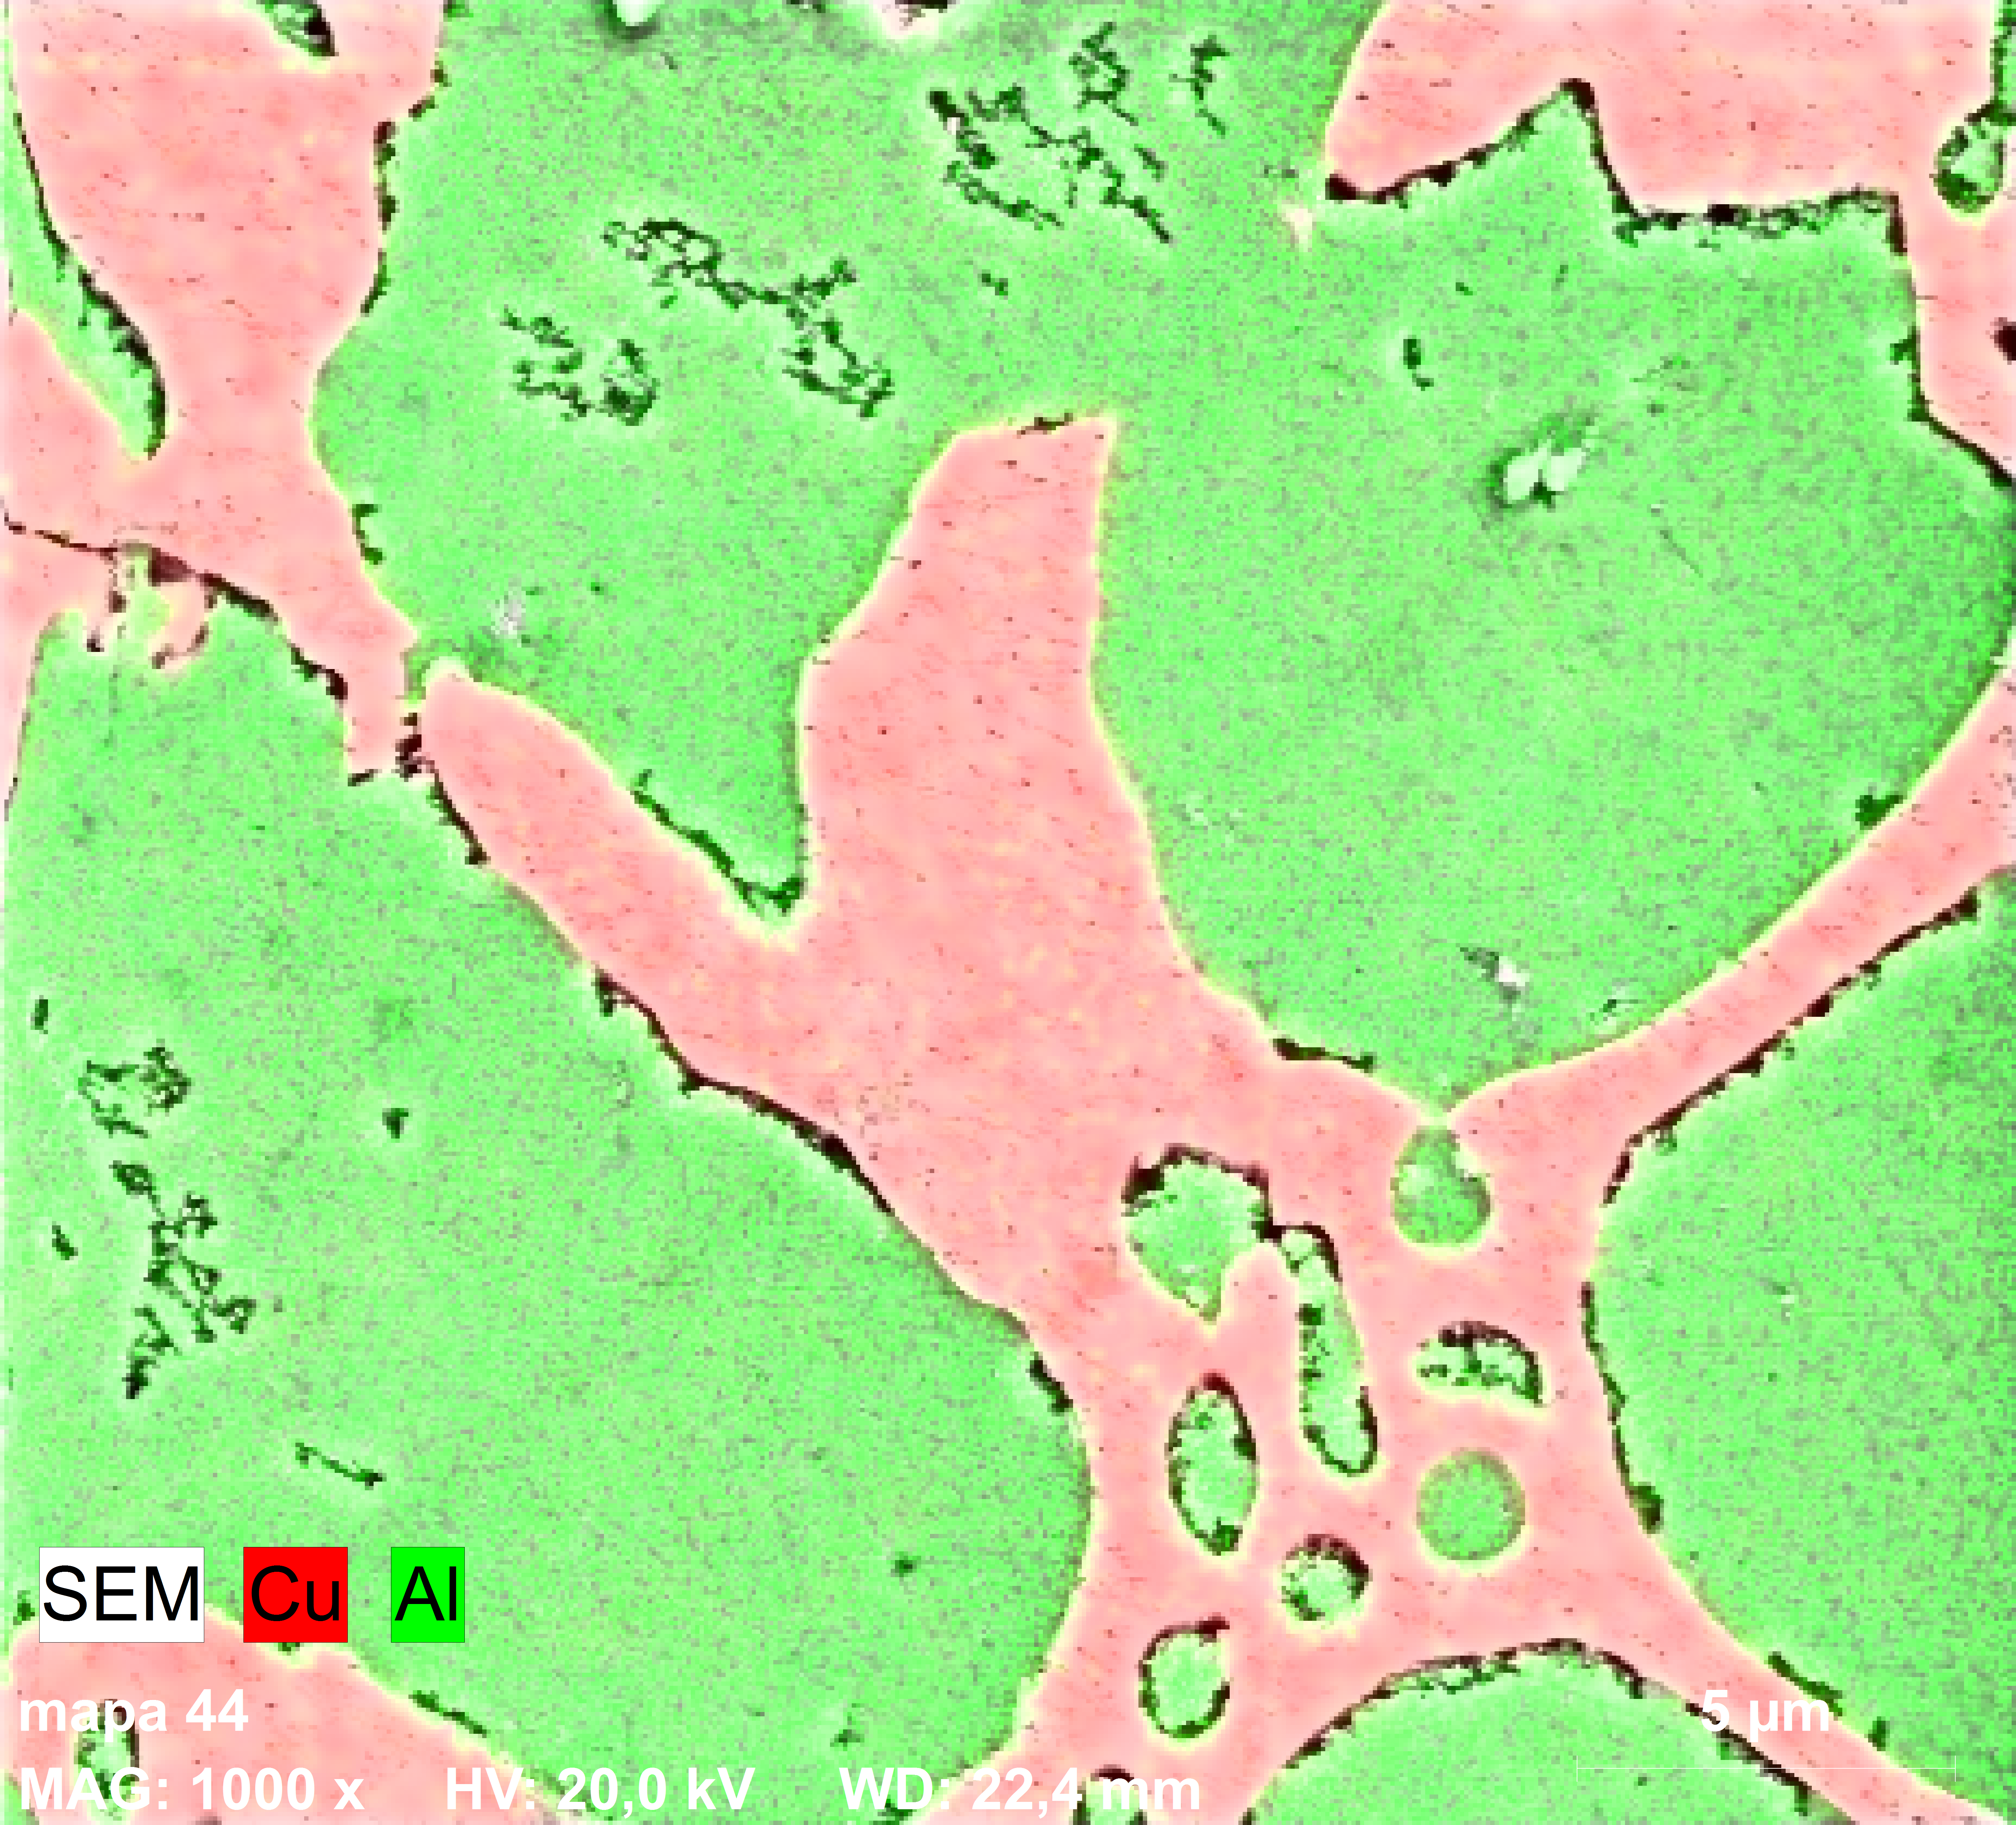
\includegraphics[width=8cm]{graficos/vz2_2D.png}
\caption{2D sken vzorku 2}
\label{o:vz2_2D}
\end{figure}


%Diskuze výsledků
\section*{Diskuze}
Při kvantitativní analýze RTG spektra jsme odhalili kromě uvedených prvků také v malém množství kyslík a uhlík. To považujeme za znečištění povrchu vzorku a ze zpracování jsme je vyloučili.


Tím, že jsme delší dobu měli zaostřeno na jedno místo, jsme vzorek kontaminovali a po oddálení mělo zasažené místo výrazně slabší intenzitu na SE i BSE detektoru, přestože předtím tomu tak nebylo.

%Závěr
\section*{Závěr}
Analýzou RTG spektra jsme určili chemické složení české padesátikoruny. Vnější mezikruží je z měďi, vnitřní kruh je slitina mědi a zinku. Tyto dvě části jsou spojené vrstvou železa.

Také jsme určili složení neznámého vzorku. Skládal se ze dvou fází, jedna byla téměř čistý hliník a druhá byla slitina hliníku a měďi (viz tabulka \ref{t:vz02_a}).


\printbibliography[title={Seznam použité literatury}]

\end{document}